\section{OBJET ET DOMAINE D'APPLICATION}
\subsection{Objet}
Cette procédure décrit le processus de découpage d'un système en sous système.
Elle est applicable et indépendante de la nature du projet et permet d'unifier la documentation de projet 
au sein de notre société, et d'en améliorer la qualité. Elle constitue un support non négligeable pour le chef de projet voire
indispensable. Elle représente un gain de temps considérable et une quantité d'expérience facilitant au chef de projet la tache de découpage 
d'un système complexe en plusieurs sous-systèmes en introduisant les étapes et les critères essentiels à la répartition d'un système en sous-systèmes
couvrant la totalité des attentes.

\subsection{Domaine d'application}
Cette procédure s'applique à tout système aussi complexe soit-il dans le cadre d'un projet de la société, sauf dérogation particulière accordée par le responsable qualité,
et ce dans un souci d'unifier et d'améliorer la documentation de projet de notre société.


\section{ABBREVIATION ET TERMINOLOGIE}

\begin{itemize}
\item[CdP:] Chef de Projet
\item[RQ: ] Responsable Qualité
\item[PMP: ] Plan de Management de Projet
\end{itemize}


\section{DOCUMENTS APPLICABLES ET DOCUMENTS DE REFERENCE}
\subsection{Documents applicables}
\begin{itemize}
\item Le PMP réalisé par le chef de projet, la procédure s'applique pour découper les systèmes en lots.
\item Document de découpage du système en sous-systèmes.
\end{itemize}

\subsection{Documents de référence}
\begin{itemize}
\item Best practice pour la rédaction d'une procédure rédigée par Baptiste LECORNU, responsable qualité.
\item Chapitre 13 du cours de qualité logiciel réalisé par Mr Régis AUBRY.
\item Manuel du chef de projet réalisé par Mr Youssef AMGHAR et Mr Régis AUBRY.
\end{itemize}


\section{PROCEDURE}
Le processus de découpage d'un système en sous-système a la forme suivante:

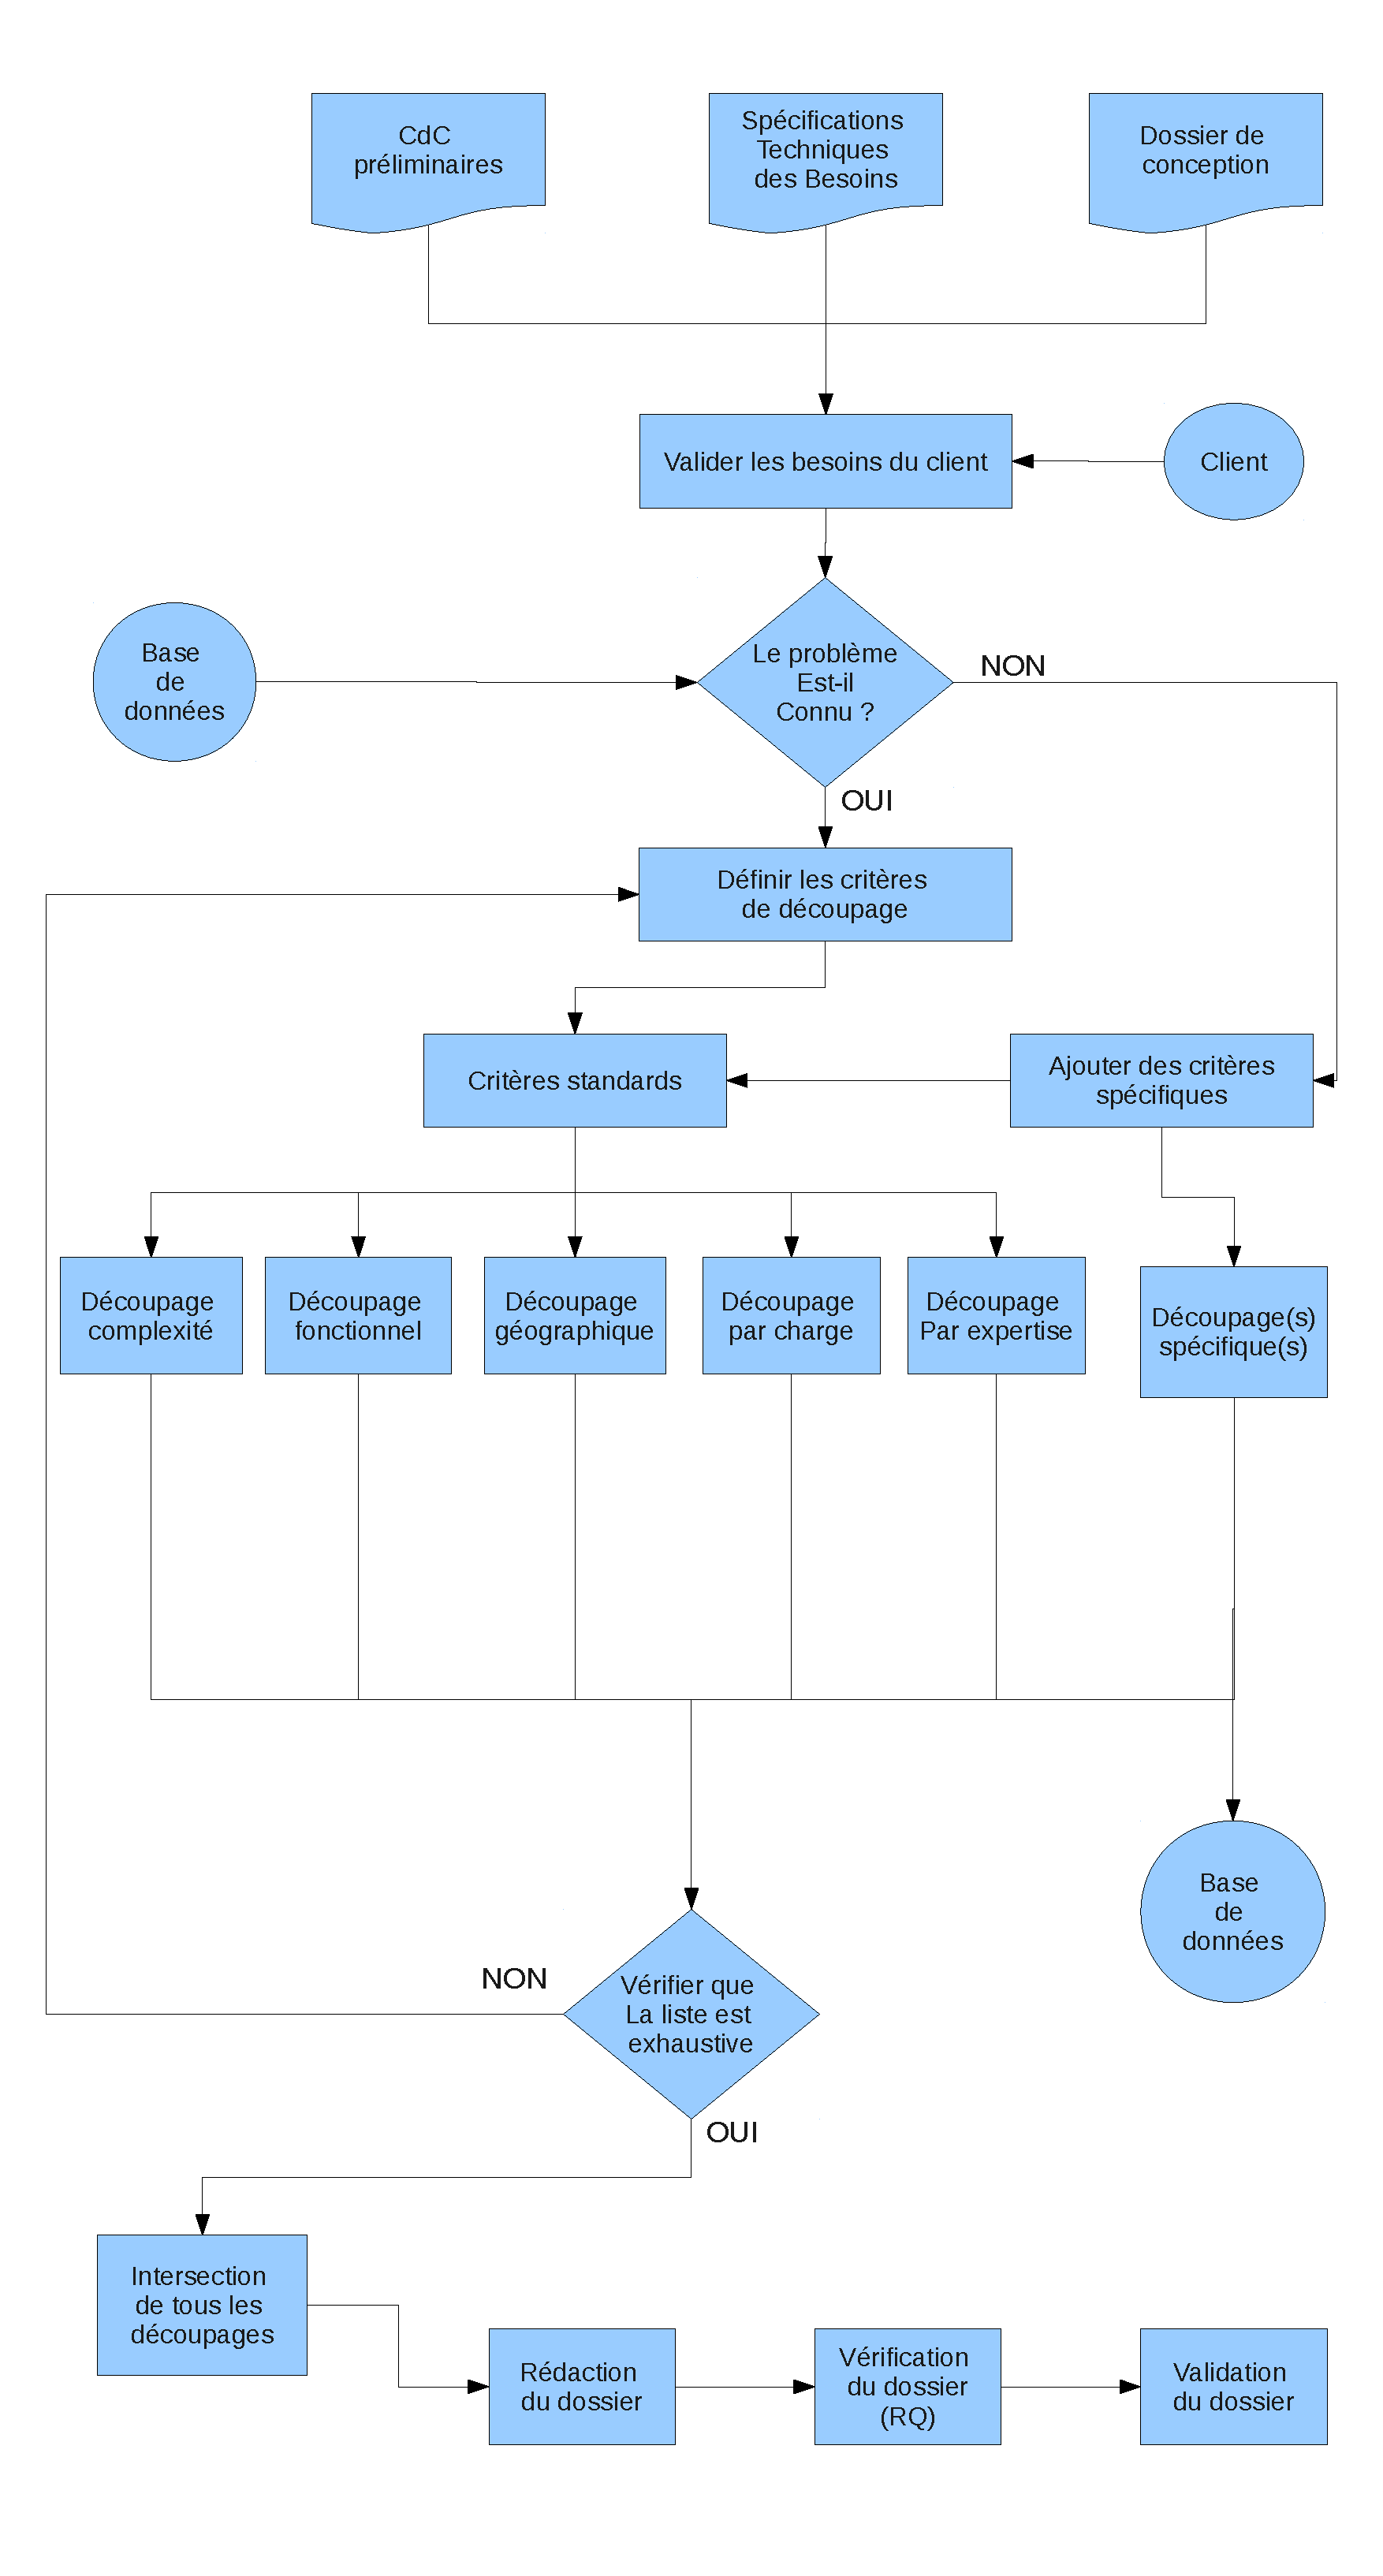
\includegraphics[width=0.9\textwidth]{./logigramme.pdf}
\begin{description}
\item[Valider les besoins du client]
Il s'agit de vérifier la cohérence des résultats afin de s'assurer que ces derniers correspondent bien aux besoins du client. Un découpage en
sous-systèmes ne peut être correct que si le système global est en corrélation avec les exigences initiales. 
\item[Le problème est-il connu ?] Cette vérification consiste à trouver des similarités avec des projets "déja vus" . Ceci permet d'exploiter l'apport d'une expérience non négligeable.
Elle permet ainsi de faire une économie de temps et de minimiser les risques d'un mauvais découpage. Cette expérience est répertoriée dans une base de donnée constamment mise à jour de manière incrémentale.
\item[Définir les critères de découpage]
Il s'agira de définir des critères standards de découpage associés à d'autres critères spécifiques au projet en question. On retrouve parmi les critères :\\
\begin{itemize}
\item Découpage complexité \\ Un critère très important à prendre en compte est la complexité du système. Il permet d'avoir une idée sur un découpage basé uniquement sur la complexité.\\
\item Découpage fonctionnel \\ C'est un critère des plus intuitifs, il permet d'avoir des sous-systèmes fonctionnels.\\
\item Découpage géographique \\ Un critère étroitement lié au déploiement du système. Il permet à la fois de considérer la dimension géographique dans le découpage durant la phase de réalisation que durant le déploiement. \\
\item Découpage par charge \\ Une évaluation de la charge de travail permet également d'avoir des sous-systèmes évaluant les charges et les ressources nécessaires. \\
\item Découpage par expertise \\ Des domaines d'études peuvent apparaitre et faire l'objet d'un découpage spécifique. Des experts métiers peuvent intervenir pour superviser ce découpage.\\
\end{itemize}
\item[Ajouter des critères spécifiques :]
Le projet peut présenter des caractéristiques telles que de nouveaux critères de découpages doivent être pris en compte. Les critères standards deviennent
ainsi insuffisants et doivent être compléter par de nouveaux facteurs.
\item[Découpage spécifique]
Il s'agit de faire un découpage suivant les nouveaux critères définis.
\item[Vérifier si la liste est exhaustive]
Il s'agit de vérifier si l'ensemble des critères (standards et / ou spécifiques) recouvre de manière globale le système initial.
\item[Intersection de tous les découpages]
A l'issue des differents découpages, on fait un tableau récapitulatif en pondérant les differents critères. On fait ainsi l'intersection de tous les découpage
pour obtenir un découpage du système en sous-systèmes.
\item[Rédaction du dossier]
Il s'agit de faire une synthèse du découpage et de produire le document illustrant ce découpage.
\item[Vérification du dossier]
Le responsable qualité vérifie puis valide le dossier.
\item[Validation du dossier]
Le chef de projet valide le dossier.
\end{description}
	   


 
